\newpage
\subsection{Technologie Versionen}
Hier sollen die einzelnen Technologien im Einzelnen beschrieben werden.
Sowie ihre geplante Funktion in unserem Projekt.
In der unten angegebenen Liste soll ein Überblick über die im Projekt verwendeten Technologien bereitstellt gestellt werden.

\begin{table}[H]
    \begin{center}
        \begin{tabular}{|c|c|}
            \hline
            
\includegraphics[width=0.1\textwidth]{bilder/technologien/NodeJS.png}    &
            \multirow[c]{1}[1]{*}[20pt]{Node.js 16.13.0 LTS}                           \\
            \hline
            
\includegraphics[width=0.1\textwidth]{bilder/technologien/Angular.png}   &
            \multirow[c]{1}[1]{*}[20pt]{Angular 13.0.1}                                \\
            \hline
            
\includegraphics[width=0.1\textwidth]{bilder/technologien/Socket.io.png} &
            \multirow[c]{1}[1]{*}[20pt]{Socket.io 4.3.2}                               \\
            \hline
            
\includegraphics[width=0.1\textwidth]{bilder/technologien/mongoDB.png}   &
            \multirow[c]{1}[1]{*}[20pt]{MongoDB Community Edition 5.0.3}               \\
            \hline
            
\includegraphics[width=0.1\textwidth]{bilder/technologien/KeyCloak.png}  &
            \multirow[c]{1}[1]{*}[20pt]{KeyCloak 15.0.2}                               \\
            \hline
            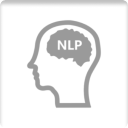
\includegraphics[width=0.1\textwidth]{bilder/technologien/NLP.png}       &
            \multirow[c]{1}[1]{*}[20pt]{NLP.js 4.22.2}                                 \\
            \hline
        \end{tabular}
        \caption{Technologie Liste}
        \label{tab:Technologie Liste}
    \end{center}
\end{table}


\subsubsection{Node.js 16.13.0 LTS}
Als Basis für Angular, den Chatbot und Keycloak nutzen wir eine LTS Version von Node.js.
Auf dem Node.js Server verwenden wir zusätzlich die Express Erweiterung,
um eine Kommunikation zu den Servern herstellen zu können.
Für uns war sehr wichtig, dass wir eine sehr stabile Basis für die Anwendung,
die wir entwickeln haben.
Deswegen haben wir uns ebenfalls informiert, ob alle geplanten oder in Frage kommenden Technologien mit der LTS Version kompatibel sind.
Nach unserem derzeitigen Stand empfehlen die Entwickler der Bibliotheken und Frameworks eine LTS Version von Node.js zu verwenden.
Bildquelle:\cite{nodejsicon}


\subsubsection{Angular 13.0.3}
Wir verwenden Angular für die Frontend-Entwicklung.
Angular ist die Basis, um das Chat- und das Admin-Interface zu erstellen.
Um unsere UIs noch effektiver zu gestalten, werden wir vereinzelt auf Angular Material zurückgreifen.
Dort gibt es zu häufig genutzten UI Komponenten "Code Snippets", die ausführlich getestet wurden.
Bildquelle:\cite{angularicon}

\subsubsection{Socket.io 4.3.1}
In unserem Projekt nutzen wir Socket.io, um eine bidirektionale Kommunikation zwischen dem Bot und
der Benutzeroberfläche herzustellen.
Es ermöglicht uns, dass ein User mit dem Chatbot ohne merkbare Verzögerung chatten kann.
Bildquelle:\cite{socketioicon}

\subsubsection{MongoDB Community Edition 5.0.3}
Wir haben uns für die Datenbank mongoDB entschieden, da es ein sehr einfaches Datenbank Modell bereitstellt.
MongoDB ist eine NoSql Datenbank, wodurch auch der Verwaltungsaufwand der Datenbank minimiert wird.
In der Datenbank wird der Korpus des Chatbots gespeichert.
Bildquelle:\cite{mongodbicon}

\subsubsection{KeyCloak 15.0.2}
In unserem Projekt verwenden wir KeyCloak, damit sich der Admin sicher in das Admin-Webinterface einloggen kann.
Zusätzlich werden wir das Shibboleth Single-Sign-On Verfahren von der Hochschule integrieren.
Damit Hochschulangehörige die Möglichkeit haben sich mit ihrem Hochschul-Account einloggen zu können.
Dadurch können wir zusätzlich begrenzen welche Personengruppen auf welche Daten Zugriff haben.
Bildquelle:\cite{keycloakicon}

\newpage
\subsubsection{RegEx}
Wir haben in unserem Projekt anfangs aus Sicherheitsgründen RegEx eingeplant.
RegEx dient in unserem Projekt als Fallback.
Um ein Scheitern des Projektes zu verhindern, falls NLP.js sich nicht in unser Projekt integrieren lassen sollte.
Damit der Chatbot dennoch Begriffe und Sätze verstehen kann.
Nach unserem derzeitigen Stand brauchen wir nicht auf eine RegEx Implementation zurückzugreifen,
da NLP.js sich sehr gut in unser Projekt integrieren lässt. 

\noindent \newline Als Beispiel für den Satz "Wie geht es dir?".
Müsste ein User oder Admin folgenden RegEx Befehl integrieren:\\
\newline \verb/(Wie|wie)\s*geht\s*es\s*dir\s*\?/ \\
\newline Damit man nach ''Wie/wie geht es dir ?'' mit und ohne Leerzeichen prüfen kann.\\
Bildquelle:\cite{regexicon}

\subsubsection{NLP.js 4.22.9}
Damit wir NLP.js nutzen können benötigen wir eine LTS Version von Node.js.
Diese Begrenzung haben wir zusätzlich in die Technologie Entscheidung einbezogen.
Indem NLP.js ab der Version 4 und höher modular ist. Wird uns ermöglicht leichter eigene Module/Plugins
für das Framework zu schreiben.
Dadurch können wir einen ChatBot mit verbesserter Spracherkennung gestalten.
Bildquelle:\cite{nlpicon}